\chapter{Estratégia de Abertura}\label{chap:6:estrat_abertura}

Para se tornar um jogador forte de Go, é necessário desenvolver duas habilidades:

\vspace{.25cm}

\begin{enumerate}[leftmargin=2.5cm,rightmargin=2cm]
    \item \textbf{leitura} à frente do tabuleiro atual, movimento por movimento, e previsão de resultados de embates locais;
    \item \textbf{intuição} sobre o que está acontecendo no tabuleiro como um todo.
\end{enumerate}

\vspace{.25cm}

O balanço aproximadamente igualitário entre qualidades intuitivas e analíticas é grande parte da atratividade do Go. Na abertura, quando o tabuleiro consiste de majoritariamente espaço vazio, é intuição, e uma base de dados de conhecimento geral, que toma um papel dominante.

\begin{wrapfigure}{r}{100mm}
    \vspace{-30pt}
    \begin{center}
        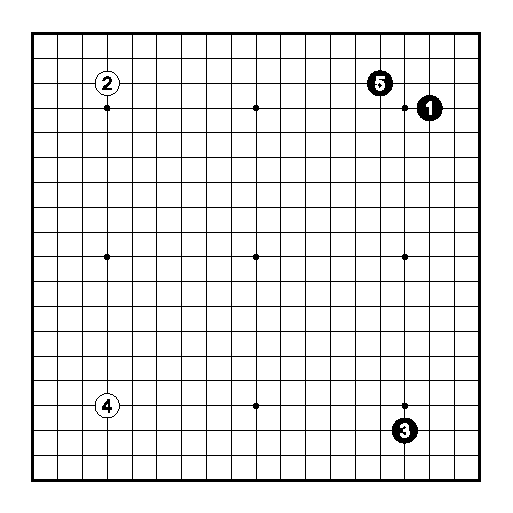
\includegraphics{6 - Dia 1}
        \caption*{\emph{Dia.\@~1 (1-5)}}
    \end{center}
    \vspace{-30pt}
\end{wrapfigure}

No tabuleiro $19\times19$, o tamanho oficial, é difícil de se assegurar território no início, então a partida usualmente começa com os jogadores espaçando suas pedras para formar grandes armações dentro das quais eles poderão brigar vantajosamente no futuro.

\emph{Dia.\@~1 a 3} mostra uma abertura típica no tabuleiro $19\times19$.

É geralmente muito mais fácil de se estabelecer bases nos cantos, como Preto e Branco o fazem com 1 a 4 no \emph{Dia.\@~1}. Uma ou duas pedras por canto é suficiente. Com 5, Preto estabelece um enclausuro de canto. Esse movimento delimita e vigia o território no canto. Não é ainda território seguro, uma vez que Branco possui múltiplas maneiras de invadi-lo. Mas Preto terá a vantagem em qualquer luta que se irromper ali. O tempo para a invasão branca será, assim, um fator crítico.

Aproximar-se do canto com Branco 6 no \emph{Dia.\@~2}, onde Preto possui somente uma pedra, é uma boa jogada. Isso frequentemente provoca lutas, como o curto conflito que se segue. Nos movimentos de 7 a 12, Preto assegura  o canto enquanto Branco constrói uma posição à direita. Essa sequência é um dos padrões-referência conhecidos como josekis.

\begin{figure}[h!]
    \centering
    \begin{subfigure}[t]{.495\textwidth}
        \centering
        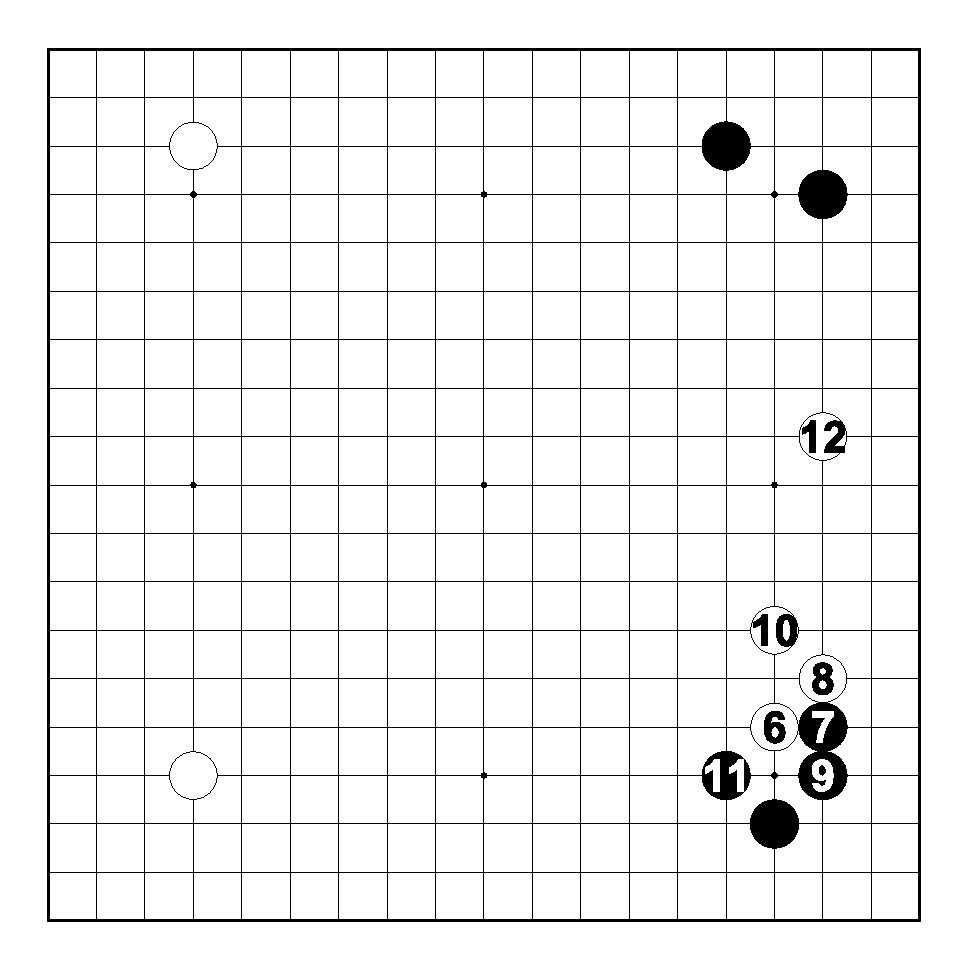
\includegraphics[width=.9\textwidth]{6 - Dia 2}
        \caption*{\emph{Dia.\@~2 (6-12)}}
    \end{subfigure}
    \begin{subfigure}[t]{.495\textwidth}
        \centering
        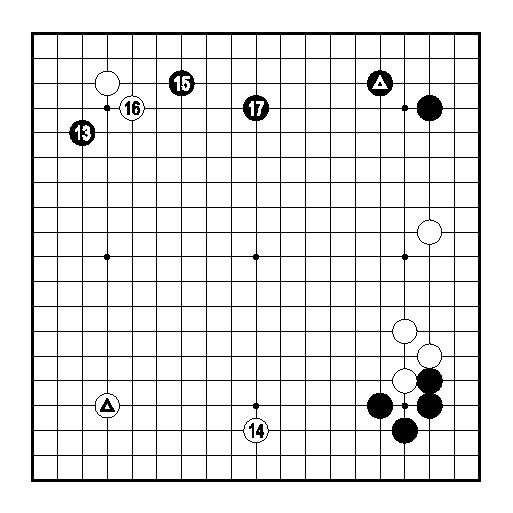
\includegraphics[width=.9\textwidth]{6 - Dia 3}
        \caption*{\emph{Dia.\@~3 (13-17)}}
    \end{subfigure}
\end{figure}

Preto 13 no \emph{Dia.\@~13} é outro exemplo de outra aproximação. Branco 14 forma uma armação esparsa no canto inferior esquerdo do tabuleiro a partir da pedra branca marcada. A terceira ou a quarta linha é a melhor para extensões como esta. Preto desenvolve uma armação no topo com 15 e 17. Note Preto 17 na quarta linha, e Preto 15 e a pedra preta marcada na terceira linha. Isso constitui um balanço ideal de jogadas altas e baixas. As pedras na terceira linha defendem os flancos da posição preta enquanto que a pedra na quarta linha expande seu território para o centro.

\pagebreak

\section{A Primeira Prioridade: Estabelecer uma Presença no Canto}

A abertura de uma partida de Go geralmente se inicia com ambos os lados estabelecendo presenças nos cantos. Os pontos a seguir são os cinco de referência que um jogador usualmente ocupa com seus primeiros movimentos.

\emph{Dia.\@~1. O ponto 3-3.} O intuito de Preto 1 no ponto 3-3 --- também conhecido como \emph{san-san} --- é assegurar o território no canto, apesar de que esse movimento não fornece muita influência no centro.

\begin{figure}[h!]
    \centering
    \begin{subfigure}[t]{.3\textwidth}
        \centering
        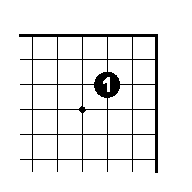
\includegraphics[trim={7cm 7cm 0cm 0cm},clip,width=.9\textwidth]{6 - Corner - Dia 1}
        \caption*{\emph{Dia.\@~1 O ponto 3-3}}
    \end{subfigure}
    \hfill
    \begin{subfigure}[t]{.3\textwidth}
        \centering
        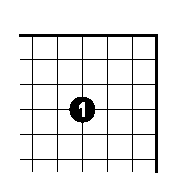
\includegraphics[trim={7cm 7cm 0cm 0cm},clip,width=.9\textwidth]{6 - Corner - Dia 2}
        \caption*{\emph{Dia.\@~2 O ponto-estrela}}
    \end{subfigure}
    \hfill
    \begin{subfigure}[t]{.3\textwidth}
        \centering
        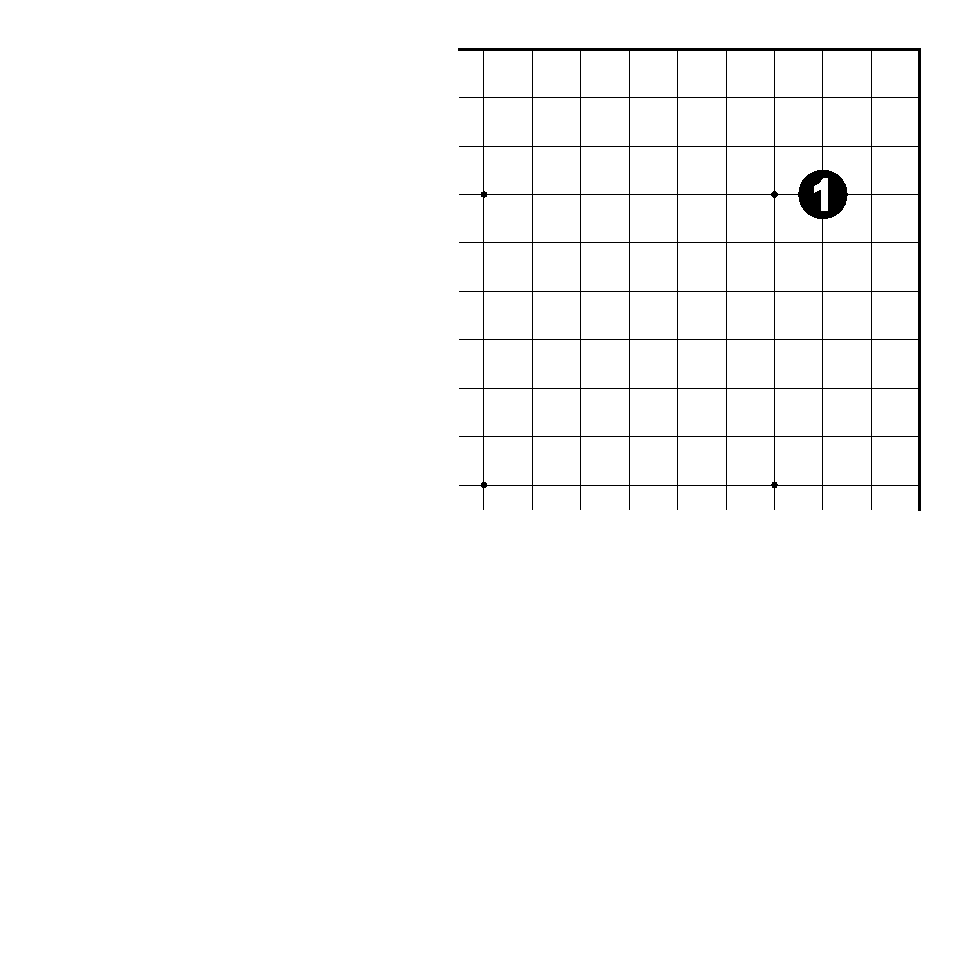
\includegraphics[trim={7cm 7cm 0cm 0cm},clip,width=.9\textwidth]{6 - Corner - Dia 3}
        \caption*{\emph{Dia.\@~3 O ponto 3-4}}
    \end{subfigure}
\end{figure}

\emph{Dia.\@~2. O ponto-estrela.} Por ter jogado no ponto 4-4 --- também conhecido como ponto-estrela --- com 1, Preto almeja influência no centro.

\emph{Dia.\@~3. O ponto 3-4.} Quando Preto joga 1 no ponto 3-4 (\emph{komoku}), ele espera ganhar território ao longo do lado direito assim como algo no canto.

\emph{Dia.\@~4. O ponto 5-3.} Preto 1 no ponto 5-3 (\emph{mokuhazushi}) enfatiza o lado. Preto está disposto a conceder a maior parte do canto para Branco.


\begin{figure}[h!]
    \centering
    \begin{subfigure}[t]{.3\textwidth}
        \centering
        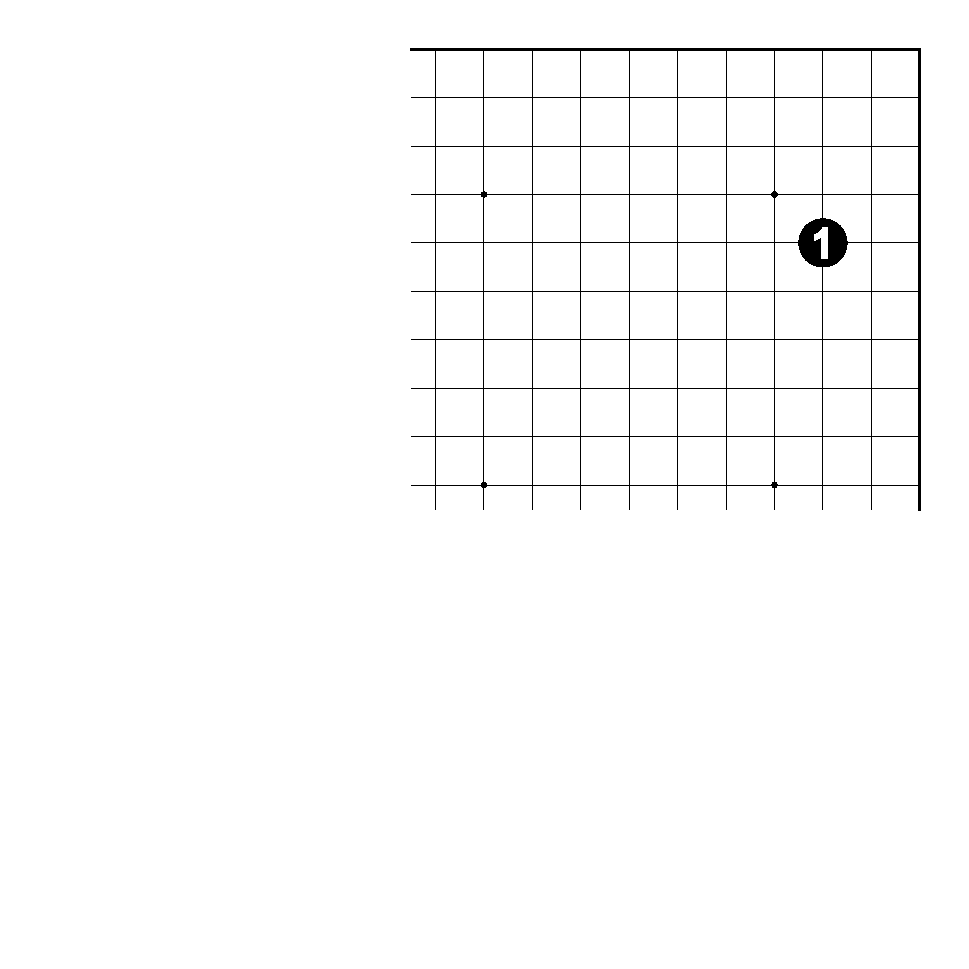
\includegraphics[trim={7cm 7cm 0cm 0cm},clip,width=.9\textwidth]{6 - Corner - Dia 4}
        \caption*{\emph{Dia.\@~4 O ponto 5-3}}
    \end{subfigure}
    \hspace{1cm}
    \begin{subfigure}[t]{.3\textwidth}
        \centering
        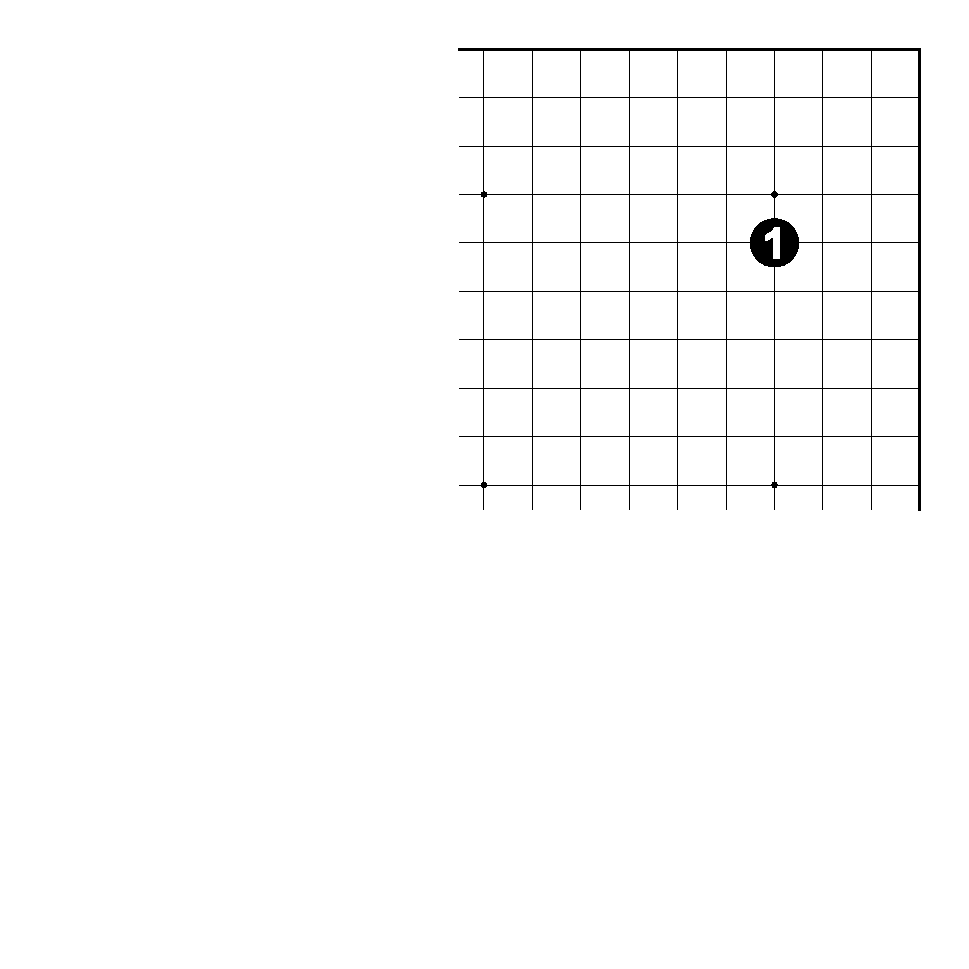
\includegraphics[trim={7cm 7cm 0cm 0cm},clip,width=.9\textwidth]{6 - Corner - Dia 5}
        \caption*{\emph{Dia.\@~5 O ponto 5-4}}
    \end{subfigure}
\end{figure}

\emph{Dia.\@~5. O ponto 5-4.} Preto 1 no ponto 5-4 (\emph{takamoku}) concede o canto ao Branco. Ele almeja influência no centro e ao longo dos lados.

\pagebreak

\section{Movimentos de Aproximação}

Depois de os jogadores terem ocupado os cantos, é praxe atacá-los ou desafiá-los. Tais movimentos são conhecidos como movimentos de aproximação.

Uma pedra no 3-3 vai geralmente ser atacada por um movimento no ponto 4-4 --- Branco 1 no \emph{Dia.\@~6}. Com movimentos até Branco 7, Preto assegura o território no canto, mas Branco ganha influência no centro. Essa sequência é um padrão estabelecido como joseki. Seria uma boa ideia memorizar esse padrão básico e outros conforme continuamos, uma vez que eles são alguns dos mais comuns que você encontrará.


\begin{figure}[h!]
    \centering
    \begin{subfigure}[t]{.3\textwidth}
        \centering
        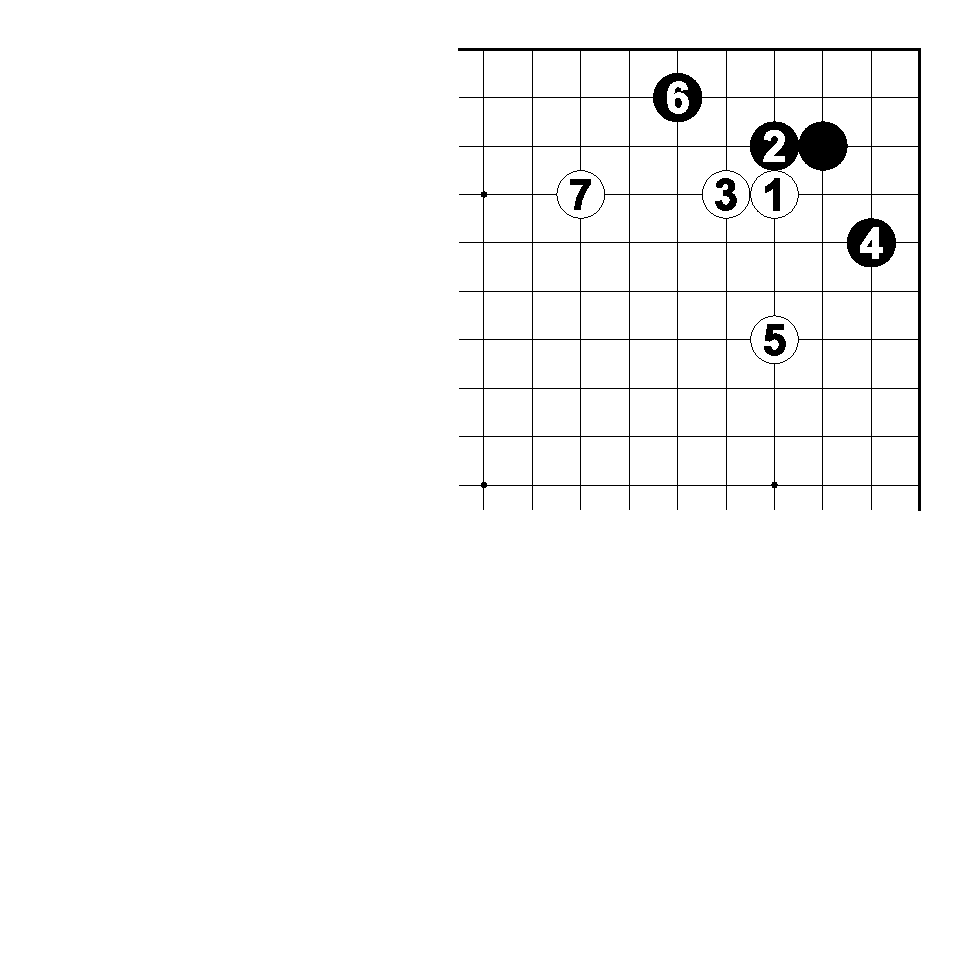
\includegraphics[trim={7cm 7cm 0cm 0cm},clip,width=.9\textwidth]{6 - Approach - Dia 6}
        \caption*{\emph{Dia.\@~6. Um joseki do ponto 3-\@3}}
    \end{subfigure}
    \hfill
    \begin{subfigure}[t]{.3\textwidth}
        \centering
        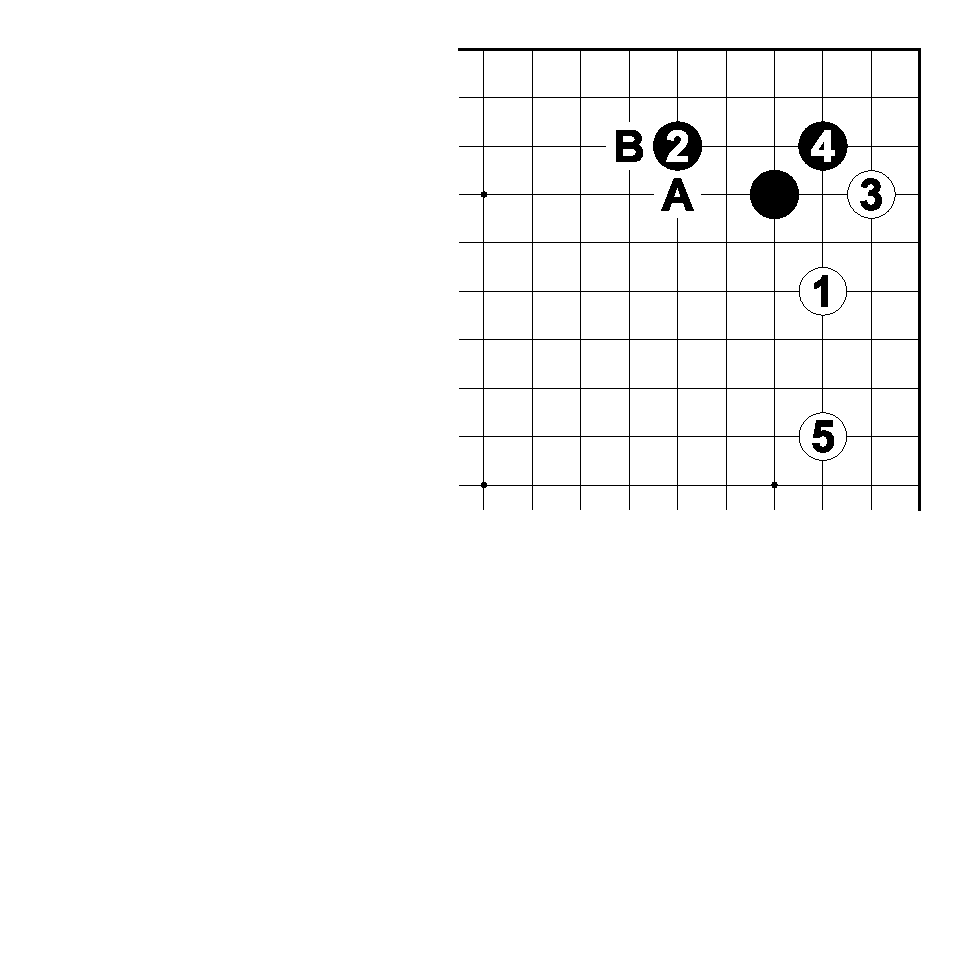
\includegraphics[trim={7cm 7cm 0cm 0cm},clip,width=.9\textwidth]{6 - Approach - Dia 7}
        \caption*{\emph{Dia.\@~7. Um joseki do ponto 4-\@4}}
    \end{subfigure}
    \hfill
    \begin{subfigure}[t]{.3\textwidth}
        \centering
        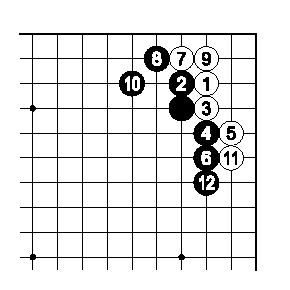
\includegraphics[trim={7cm 7cm 0cm 0cm},clip,width=.9\textwidth]{6 - Approach - Dia 8}
        \caption*{\emph{Dia.\@~8. Um joseki do ponto 4-\@4}}
    \end{subfigure}
\end{figure}

Contra uma pedra jogada no ponto 4-4, é usual se aproximar com um movimento do cavaleiro --- similar ao do cavalo no xadrez --- de Branco 1 no \emph{Dia.\@~7}. Preto 2 é a resposta típica, mas Preto 2 em \textbf{A} ou \textbf{B} também são frequentemente jogados. Branco agora continua deslizando para 3, Preto defende o canto com 4, e Branco estende dois espaços até 5. Isso também é um joseki básico.

Ao invés de 1 no \emph{Dia.\@~7}, Branco poderia também invadir o ponto 3-3 com 1 no \emph{Dia.\@~8}. A sequência até Preto 12 é outro joseki básico. Branco consegue um território blindado no canto, mas Preto obtém uma posição muito densa no exterior. Se não houver muitas pedras no tabuleiro, a densidade preta é julgada como melhor do que o território branco, portanto não é aconselhável que Branco jogue essa sequência até que o meio de jogo comece. Esse joseki enfatiza a principal fraqueza da pedra situada no ponto 4-4: ela deixa o canto aberto para invasões. No entanto, um jogador que queira prosseguir com uma estratégia que enfatize influência central vai geralmente jogar uma pedra ou no ponto 4-4 ou no ponto 5-4.

Contra uma pedra no ponto 3-4, há duas aproximações básicas: o movimento curto do cavaleiro em \textbf{A} no \emph{Dia.\@~9} e a aproximação de um espaço em \textbf{B}.

\begin{figure}[h!]
    \centering
    \begin{subfigure}[t]{.3\textwidth}
        \centering
        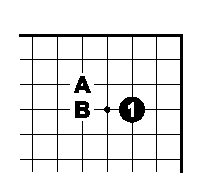
\includegraphics[trim={7cm 8cm 0cm 0cm},clip,width=.9\textwidth]{6 - Approach - Dia 9}
        \caption*{\emph{Dia.\@~9}}
    \end{subfigure}
    \hfill
    \begin{subfigure}[t]{.3\textwidth}
        \centering
        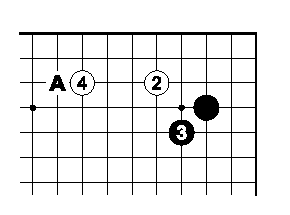
\includegraphics[trim={7cm 7cm 0cm 0cm},clip,width=.9\textwidth]{6 - Approach - Dia 10}
        \caption*{\emph{Dia.\@~10}}
    \end{subfigure}
    \hfill
    \begin{subfigure}[t]{.3\textwidth}
        \centering
        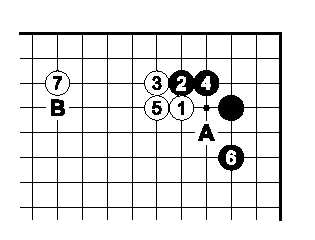
\includegraphics[trim={7cm 7cm 0cm 0cm},clip,width=.9\textwidth]{6 - Approach - Dia 11}
        \caption*{\emph{Dia.\@~11}}
    \end{subfigure}
\end{figure}

Contra a aproximação curta do cavaleiro de Branco 1 no \emph{Dia.\@~10}, Preto 2 é uma resposta sólida. Branco pode responder estendendo até 3 ou mesmo tão distantemente quanto \textbf{A}.

Se Branco joga a aproximação de um espaço de 1 no \emph{Dia.\@~11}, contatar-se com Preto 2 é uma resposta popular. A sequência até Branco 7 é um joseki básico. Preto assegura o canto e Branco estabelece uma posição no topo. Preto poderia também jogar 6 em \textbf{A}, e Branco poderia jogar 7 em \textbf{B}. Compare esse joseki a movimentos como 6 a 12 no \emph{Dia.\@~2} no início desta seção sobre estratégia de abertura.

Quando Preto possui uma pedra no ponto 5-3 (a pedra marcada), Branco 1 no \emph{Dia.\@~12} é a aproximação padrão. Preto responde achatando Branco com 2 e 4. Branco assegura o território à direita com 3 e 5 e Preto estende a partir de sua parede com 6, estabelecendo uma posição no topo.

\begin{figure}[h!]
    \centering
    \begin{subfigure}[t]{.3\textwidth}
        \centering
        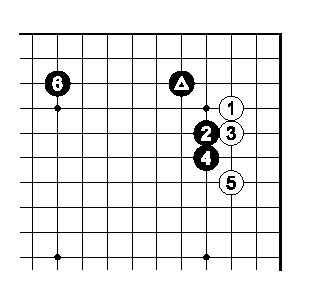
\includegraphics[trim={6cm 7cm 0cm 0cm},clip,width=.9\textwidth]{6 - Approach - Dia 12}
        \caption*{\emph{Dia.\@~12}}
    \end{subfigure}
    \hspace{1cm}
    \begin{subfigure}[t]{.3\textwidth}
        \centering
        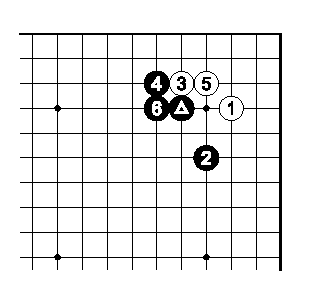
\includegraphics[trim={6cm 7cm 0cm 0cm},clip,width=.9\textwidth]{6 - Approach - Dia 13}
        \caption*{\emph{Dia.\@~13}}
    \end{subfigure}
\end{figure}

O intuito de se jogar uma pedra preta no ponto 5-4 (a pedra marcada) no \emph{Dia.\@~13} é ganhar influência no centro. Quando Branco se aproxima com 1, Preto joga 2, confinando Branco ao canto. Com a sequência até 7, Branco garante o território no canto, e Preto ganha a influência no centro.

\pagebreak

\section{Pinças}

Quando um lado faz um movimento de aproximação, o outro frequentemente segue com uma pinça.

Após Branco se aproximar com a pedra no 4-4 com 1 no \emph{Dia.\@~14}, Branco pode jogar uma pinça com 2. (Pinças de \textbf{A} a \textbf{E} também são possíveis e frequentemente jogadas.) Em resposta, Branco geralmente invade o canto com 3 no \emph{Dia.\@~15}. A sequência até Branco 11 é um joseki. Branco ganha território no canto, e Preto consegue uma posição densa no entorno.

\begin{figure}[h!]
    \centering
    \begin{subfigure}[t]{.3\textwidth}
        \centering
        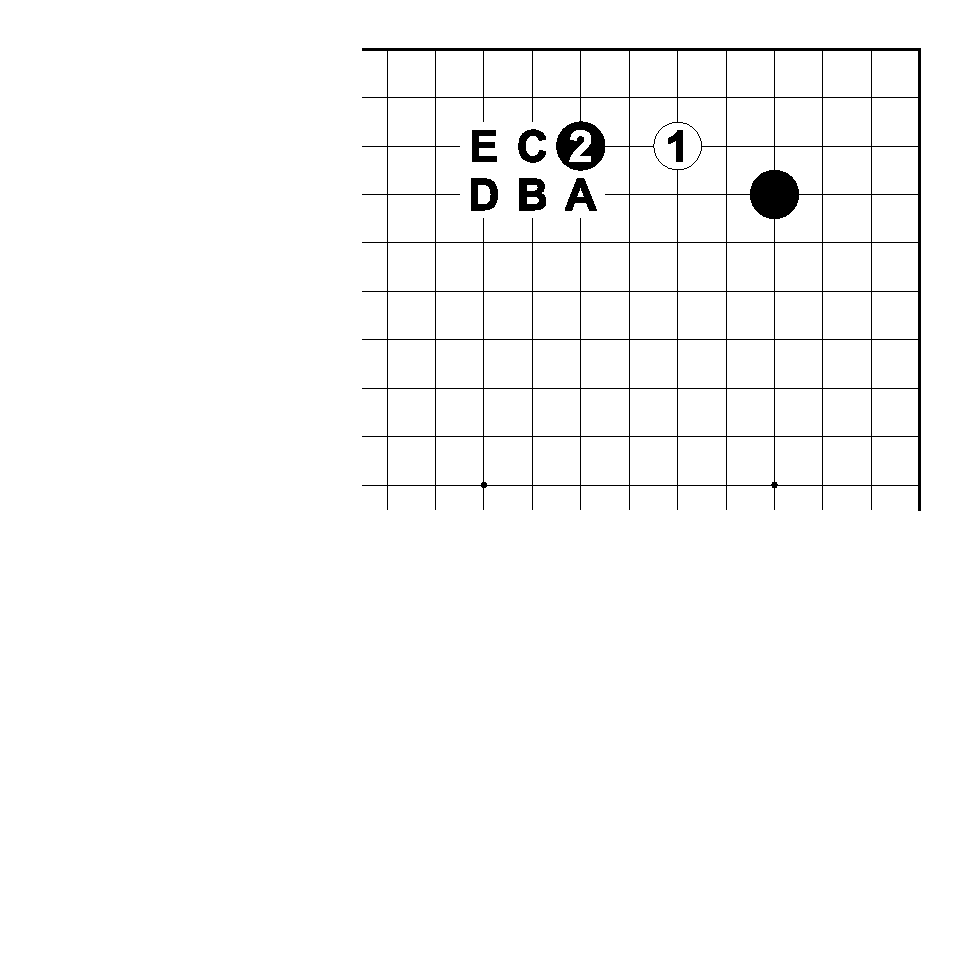
\includegraphics[trim={6cm 7cm 0cm 0cm},clip,width=.9\textwidth]{6 - Pincers - Dia 14}
        \caption*{\emph{Dia.\@~14}}
    \end{subfigure}
    \hspace{1cm}
    \begin{subfigure}[t]{.3\textwidth}
        \centering
        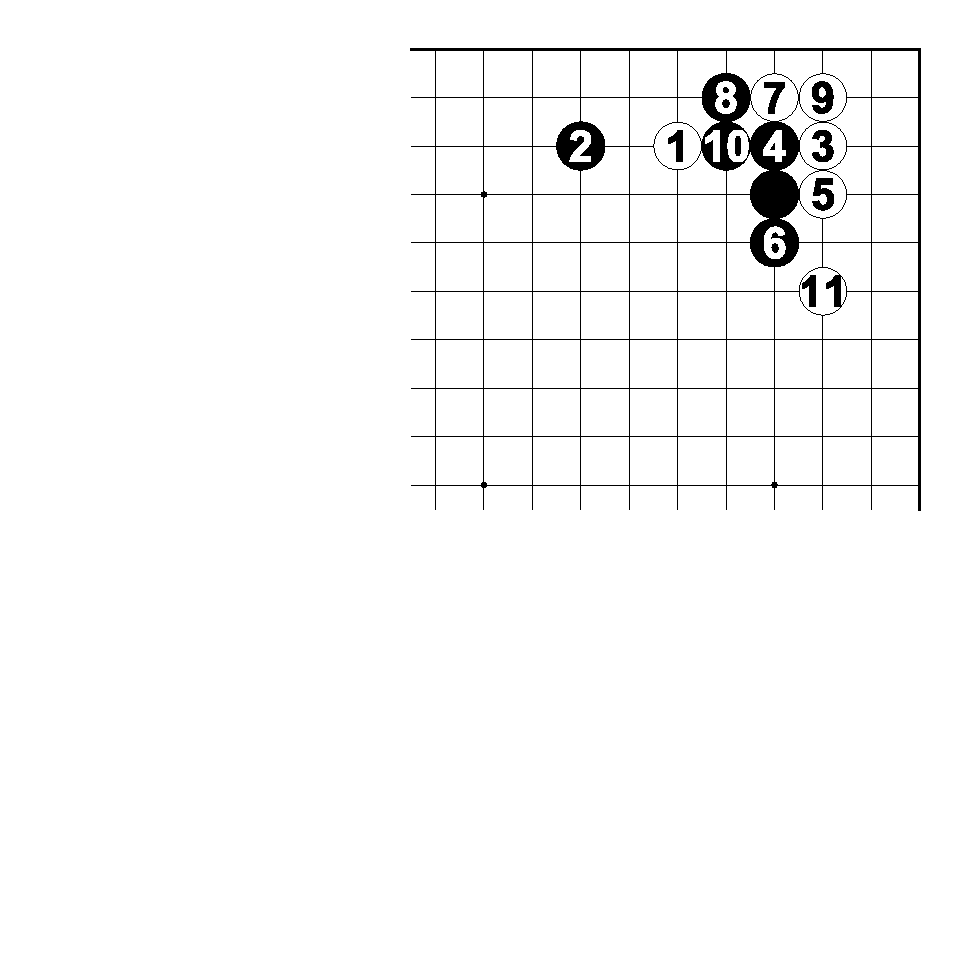
\includegraphics[trim={6cm 7cm 0cm 0cm},clip,width=.9\textwidth]{6 - Pincers - Dia 15}
        \caption*{\emph{Dia.\@~15}}
    \end{subfigure}
\end{figure}

Quando Preto possui a pedra marcada, como no \emph{Dia.\@~16}, a direção correta para Preto bloquear é por baixo com 4. Os movimentos até Preto 8 também constituem um joseki. Novamente, Branco consegue o canto, mas Preto conseguiu mapear uma armação territorial no lado superior direito com sua parede e a pedra marcada.

\begin{figure}[h!]
    \centering
    \begin{subfigure}[t]{.3\textwidth}
        \centering
        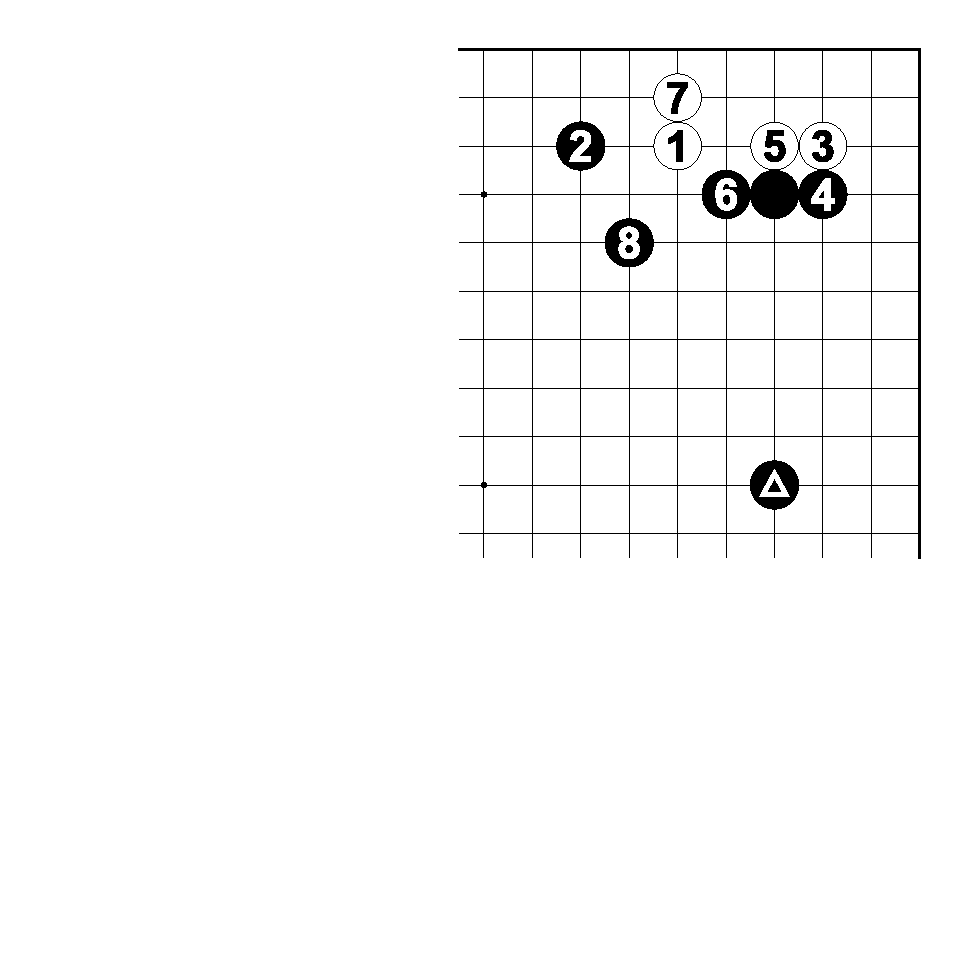
\includegraphics[trim={6cm 7cm 0cm 0cm},clip,width=.9\textwidth]{6 - Pincers - Dia 16}
        \caption*{\emph{Dia.\@~16}}
    \end{subfigure}
    \hspace{1cm}
    \begin{subfigure}[t]{.3\textwidth}
        \centering
        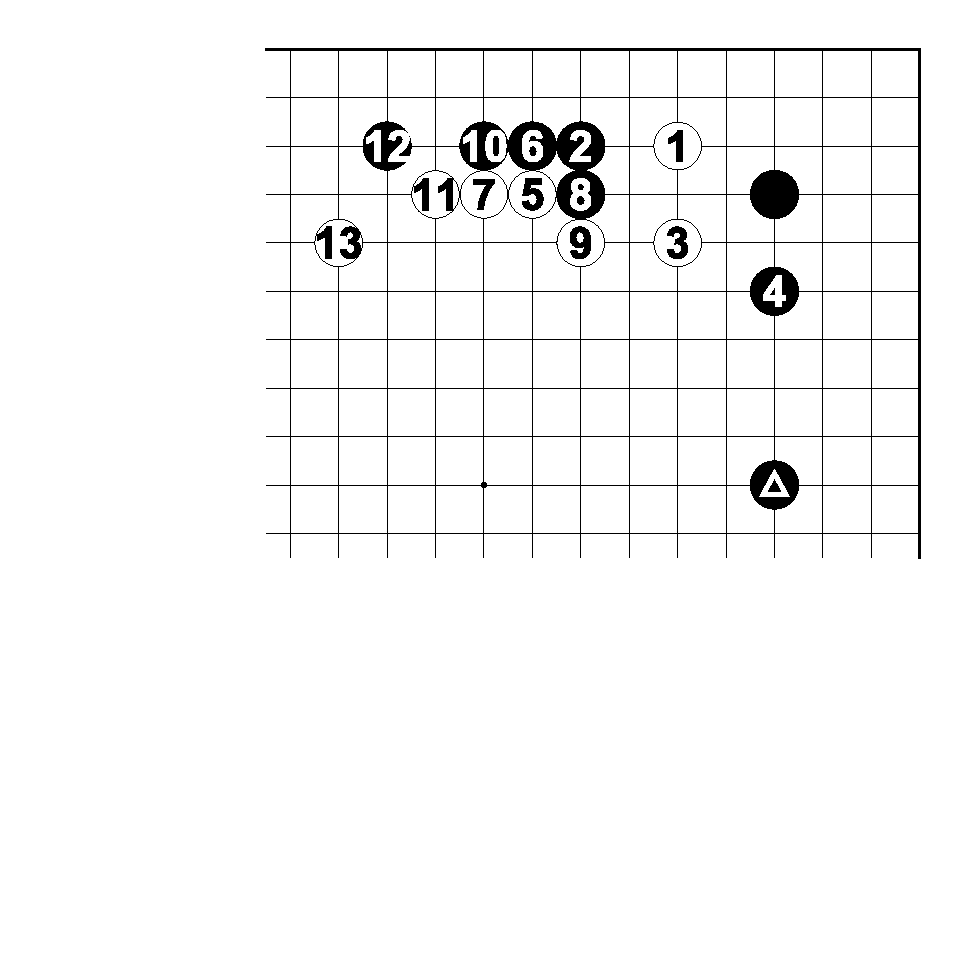
\includegraphics[trim={5cm 6cm 0cm 0cm},clip,width=.9\textwidth]{6 - Pincers - Dia 17}
        \caption*{\emph{Dia.\@~17}}
    \end{subfigure}
\end{figure}

Se Branco não estiver satisfeito com o resultado no \emph{Dia.\@~16}, em que Preto possui uma presença esmagadora no centro enquanto que suas próprias pedras se confinam ao canto, ele pode optar pela resposta 3 à Preto 2 no \emph{Dia.\@~17}. Após a sequência joseki até 13, Preto assegurou uma posição no topo e, ainda, mapeou uma esfera de influência no lado direito, mas Branco conseguiu estabelecer uma presença no centro. Branco 13 em \textbf{A} também é uma jogada tida como joseki.

No \emph{Dia.\@~18}, Branco se aproxima da pedra marcada no ponto 3-4 com 1, e Preto joga a pinça com 2. Branco sai para o centro com o movimento diagonal de 3, e Preto defende o lado direito com 4. Finalmente, Branco estabelece uma base para suas pedras deslizando até 5, e Preto delimita seu território no lado direito com a extensão até 6.

\begin{figure}[h!]
    \centering
    \begin{subfigure}[t]{.3\textwidth}
        \centering
        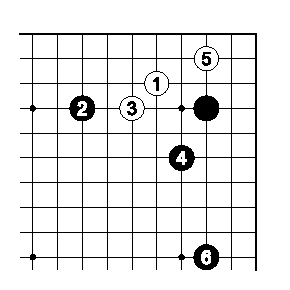
\includegraphics[trim={6cm 6cm 0cm 0cm},clip,width=.9\textwidth]{6 - Pincers - Dia 18}
        \caption*{\emph{Dia.\@~18}}
    \end{subfigure}
    \hspace{1cm}
    \begin{subfigure}[t]{.3\textwidth}
        \centering
        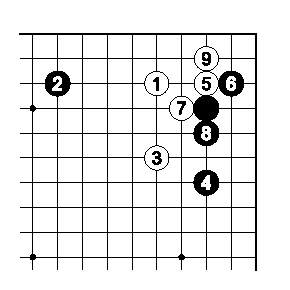
\includegraphics[trim={6cm 6cm 0cm 0cm},clip,width=.9\textwidth]{6 - Pincers - Dia 19}
        \caption*{\emph{Dia.\@~19}}
    \end{subfigure}
\end{figure}

Apesar de que um pouco distante, Preto 2 no \emph{Dia.\@~19} é também uma pinça contra 1. Branco sai para o centro com seu pulo de dois espaços em 3. Preto defende o lado direito com 4, e Branco faz uma base com suas pedras de 5 a 9.

Preto 2 no \emph{Dia.\@~19} é o mais distante que uma pedra pode ser jogada para ser denominada como pinça. Por exemplo, Preto 2 no \emph{Dia.\@~20} não é uma pinça contra a pedra branca em 1 pois Branco pode jogar a extensão ideal de 3.

\begin{figure}[h!]
    \centering
    \begin{subfigure}[t]{.3\textwidth}
        \centering
        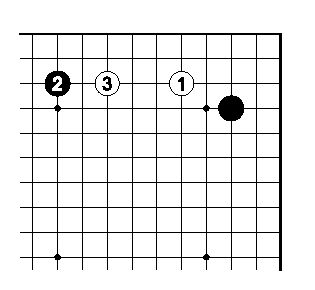
\includegraphics[trim={6cm 6cm 0cm 0cm},clip,width=.9\textwidth]{6 - Pincers - Dia 20}
        \caption*{\emph{Dia.\@~20}}
    \end{subfigure}
    \hspace{1cm}
    \begin{subfigure}[t]{.3\textwidth}
        \centering
        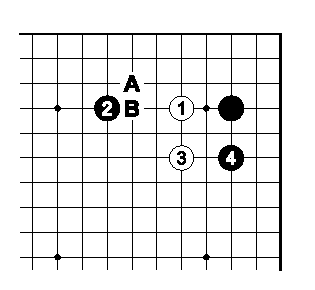
\includegraphics[trim={6cm 6cm 0cm 0cm},clip,width=.9\textwidth]{6 - Pincers - Dia 21}
        \caption*{\emph{Dia.\@~21}}
    \end{subfigure}
\end{figure}

Contra a aproximação alta de Branco 1 no \emph{Dia.\@~21}, há diversas pinças que podem ser jogadas. Preto 2, \textbf{A} e \textbf{B} são as mais comuns. Se Branco responder Preto 2 pulando ao centro com 3, Preto defenderá de maneira disciplinada e apertada o lado direito com 4.

\pagebreak

\section{Josekis}

Nas seções sobre aproximações e pinças, vários josekis básicos foram introduzidos. Esses josekis são tão básicos que eles constantemente surgem em partidas, então é uma boa ideia memorizá-los. Josekis provêm exemplos de bons movimentos que você pode aplicar a posições em seus próprios jogos, sendo assim, ao estudá-los, você gradativamente afiará sua intuição sobre o que constitui uma boa jogada.

Um bom livro para se começar a estudar josekis é \emph{38 Basic Josekis}~\cite{kosugi_bozulich_38_basic_joseki}. Conforme você se tornar mais forte, você irá querer um livro de referência mais completo no assunto. Para esse propósito, nós recomendamos a coleção de dois volumes \emph{21st Century Dictionary of Basic Josekis}~\cite{takao_shinji_21st_century_joseki_dictionary}, por Takao Shinji 9p. Apesar de que ele não contém algumas inovações recentes, outro excelente livro é o livro \emph{A Dictionary of Basic Josekis}~\cite{ishida_yoshio_basic_joseki_dictionary}, por Ishida Yoshio 9p. Ele contém muitos exemplos de jogos nos quais os josekis foram estudados e utilizados. Todos esses livros foram publicados pela Kiseido~\cite{kiseido}.

\pagebreak

\section{Enclausuros de Canto}

\begin{wrapfigure}{r}{80mm}
    \vspace{-35pt}
    \begin{center}
        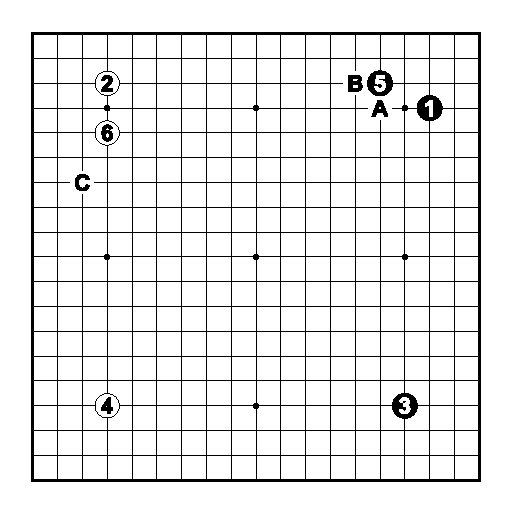
\includegraphics{6 - Corner Enclosures.eps}
        \caption*{\emph{Dia.\@~22}}
    \end{center}
    \vspace{-35pt}
\end{wrapfigure}

Ao invés de fazer uma jogada de aproximação, um jogador talvez escolha reforçar uma pedra que ele já jogou em um canto, com um enclausuro. Na abertura mostrada no \emph{Dia.\@~22}, após Branco 4, Preto faz um enclausuro de movimento de cavaleiro curto com com 5. Preto poderia também fazer o enclausuro de um espaço jogando em \textbf{A} ou o de cavaleiro longo com \textbf{B}. Essas são todas boas jogadas, mas o de cavaleiro curto é o que mais vem sendo jogado ultimamente pois tende a melhor defender o canto. O enclausuro de um espaço de Branco 6 é jogado para enfatizar o centro, mas, já que possui um flanco aberto, está vulnerável a um ataque ao redor de \textbf{C}.

\pagebreak

\section{Extensões}

Até aqui, consideramos movimentos feitos primariamente em torno do canto. Conforme a partida progride, extensões ao longo dos lados precisarão ser feitas. Extensões precisam trabalhar eficientemente. Elas deveriam não ser demasiado curtas nem demasiado longas. Há três princípios relacionados que oferecem diretivas para a criação de extensões eficientes.

\begin{itemize}
    \item[\textbf{Princípio 1}] De uma pedra só, estenda dois espaços.
        
        De uma pedra só na terceira linha, uma extensão de dois espaços é a mais eficiente. Por exemplo, Branco faz um aproximação de cavaleiro longo contra a pedra preta no ponto 3-4 com 1 no \emph{Dia.\@~23}. Se Preto defende o canto com 2, a extensão de dois espaços de Branco 3 é a resposta ideal. Isso é um joseki e possui a distinção de ser um dos mais curtos. (Outro joseki curto é mostrado no \emph{Dia.\@~10}.)
    
    \begin{figure}[h!]
        \centering
        \begin{subfigure}[t]{.3\textwidth}
            \centering
            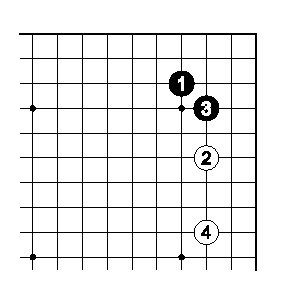
\includegraphics[trim={3cm 3cm 0cm 0cm},clip,width=.9\textwidth]{6 - Extensions - Dia 23}
            \caption*{\emph{Dia.\@~23}}
        \end{subfigure}
        \hfill
        \begin{subfigure}[t]{.3\textwidth}
            \centering
            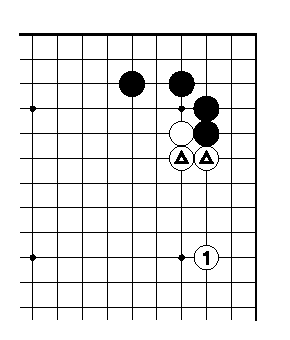
\includegraphics[trim={3cm 3cm 0cm 0cm},clip,width=.9\textwidth]{6 - Extensions - Dia 24}
            \caption*{\emph{Dia.\@~24}}
        \end{subfigure}
        \hfill
        \begin{subfigure}[t]{.3\textwidth}
            \centering
            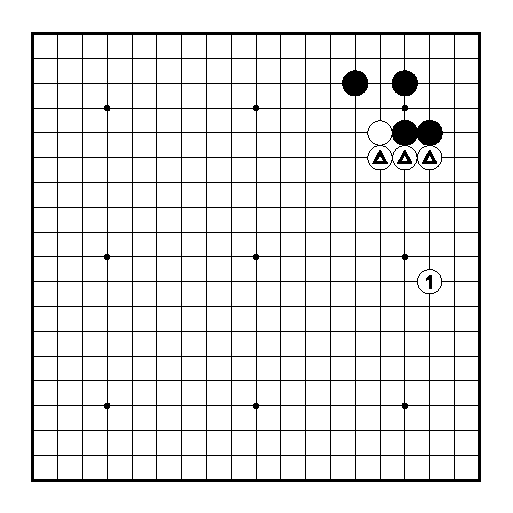
\includegraphics[trim={3cm 3cm 0cm 0cm},clip,width=.9\textwidth]{6 - Extensions - Dia 25}
            \caption*{\emph{Dia.\@~25}}
        \end{subfigure}
    \end{figure}

    \item[\textbf{Princípio 2}] De uma parede de duas pedras, estenda três espaços.
    
        No \emph{Dia.\@~24}, Branco possui uma parede de duas pedras (as pedras marcadas). A partir dessa parede, estender três espaço para 1 é o ideal. (Essa posição foi gerada a partir do joseki mostrado no \emph{Dia.\@~11}, apesar de que em uma orientação diferente.)
    \item[\textbf{Princípio 3}] De uma parede de três pedras, estenda quatro espaços. 

        No \emph{Dia.\@~25}, Branco fez uma parede de três pedras (as pedras marcadas), então ele pode estender quatro espaços até 1.
\end{itemize}

\pagebreak

\begin{wrapfigure}{r}{80mm}
    \vspace{-20pt}
    \begin{center}
        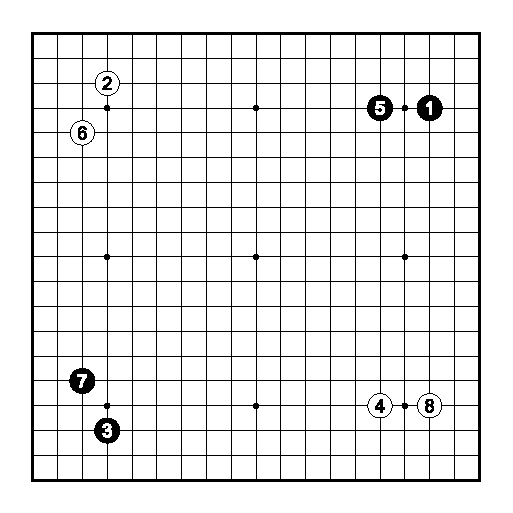
\includegraphics{6 - Extensions - Dia 26.eps}
        \caption*{\emph{Dia.\@~26}}
    \end{center}
    \vspace{-20pt}
\end{wrapfigure}

Esses princípios não são tão rígidos; eles deveriam ser interpretados como diretivas. Suas extensões precisam trabalhar não somente em consonância com suas próprias pedras mas também efetivamente para frustrar os planos do oponente.

Na abertura no \emph{Dia.\@~26}, nenhum movimento de aproximação foi feito, e cada lado tomou dois enclausuros de canto. A atenção agora se desloca para as extensões ao longo dos lados. Após Branco 8, onde está a maior extensão? O que deveria imediatemente são os dois enclausuros de canto de um espaço no lado direito, olhando um para o outro. O lado que estender de seu enclausuro primeiro tomará a iniciativa.

\begin{wrapfigure}{l}{80mm}
    \vspace{-25pt}
    \begin{center}
        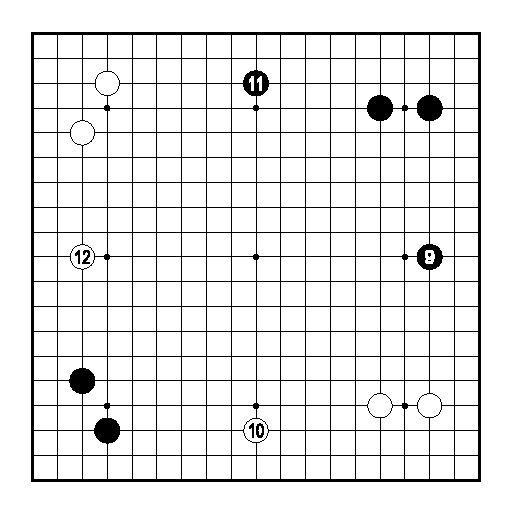
\includegraphics{6 - Extensions - Dia 27.eps}
        \caption*{\emph{Dia.\@~27}}
    \end{center}
    \vspace{-150pt}
\end{wrapfigure}

\bigskip

Por estender cinco espaços de seu enclausuro no canto superior direito com 9 no \emph{Dia.\@~27}, Preto toma a iniciativa no lado direito. Este é o ponto em que Branco também gostaria de jogar, uma que está na direção em que ambos os enclausuros emanam influência. Em geral, estender cinco espaços de um enclausuro é a norma.

Branco responde estendendo no lado inferior com 10. Esse movimento faz duas coisas: pára uma extensão preta a partir do enclausuro no canto inferior esquerdo; e protege o flanco do enclausuro branco. Preto 11 possui o mesmo significado. Branco 12 no lado esquerdo é a extensão de menor valor, dado que os enclausuros preto e branco não projetam muita influência nesta direção.

\pagebreak

\begin{wrapfigure}{r}{80mm}
    \vspace{-20pt}
    \begin{center}
        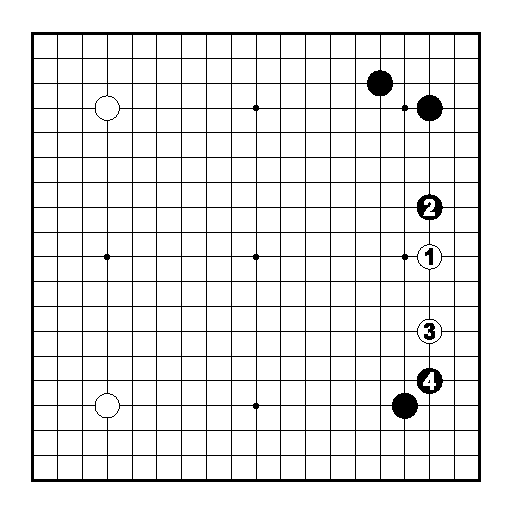
\includegraphics{6 - Extensions - Dia 28.eps}
        \caption*{\emph{Dia.\@~28}}
    \end{center}
    \vspace{-10pt}
\end{wrapfigure}

Não é sempre possível fazer uma extensão de um enclausuro de canto. No \emph{Dia.\@~28}, por exemplo, Branco joga no meio da esfera de influência preta com 1. Preto 2 é o mais longe que Preto pode estender a partir de seu enclausuro. Branco precisa construir uma base para suas pedras estendendo para 3, e Preto reforça seu canto com 4.

\begin{wrapfigure}{l}{80mm}
    \vspace{-35pt}
    \begin{center}
        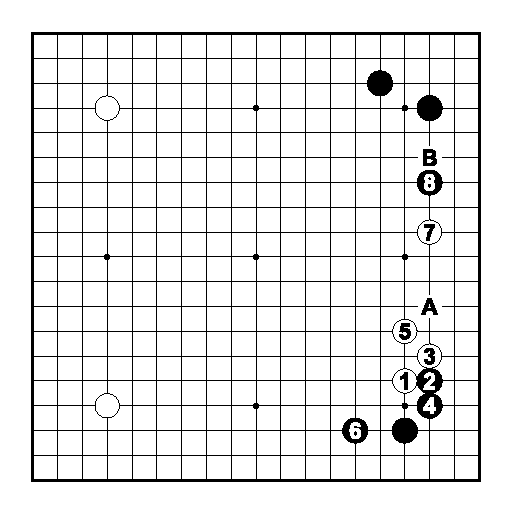
\includegraphics{6 - Extensions - Dia 29.eps}
        \caption*{\emph{Dia.\@~29}}
    \end{center}
\end{wrapfigure}

No \emph{Dia.\@~29}, Branco quer prevenir a segunda extensão de enclausuro preta no canto inferior direito, então ele faz a aproximação alta de 1. Preto contata com 2, e isso tudo resulta no joseki até Branco 7. Preto 8 talvez pareça uma extensão curta, mas, ainda assim, é uma boa jogada, porque contém a ameaça da invasão em \textbf{A}. Além disso, ela previne a jogada branca \textbf{B}, que reforçaria a posição branca no lado direito enquanto ameaçaria o enclausuro preto acima.

\bigskip

Essa é somente uma breve introdução à abertura. Para um tratamento mais completo dessa etapa da partida, recomendamos os seguintes dois livros publicados pela Kiseido: \emph{Opening Theory Made Easy}~\cite{otake_opening_theory_made_easy}, por Otake Hideo 9p; e \emph{In the Beginning}~\cite{ikure_in_the_beginning}, por Ikuro Ishigure.